%%%%%%%%%%%%%%%%%%%%%%%%%%%%%%%%%%%%%%%%%%%%%%%%%%%%%%%%%%%%%%%%%%%%%%%%%%%%%%%%%%%%%%%%%%%%%%%%%%%%%%%%%%%%%%%%%%%%%%%%%%%%%%%%%%%%%%%%%%%%%%%%%%%%%%%%%%%
% This is just an example/guide for you to refer to when submitting manuscripts to Frontiers, it is not mandatory to use Frontiers .cls files nor frontiers.tex  %
% This will only generate the Manuscript, the final article will be typeset by Frontiers after acceptance.
%                                              %
%                                                                                                                                                         %
% When submitting your files, remember to upload this *tex file, the pdf generated with it, the *bib file (if bibliography is not within the *tex) and all the figures.
%%%%%%%%%%%%%%%%%%%%%%%%%%%%%%%%%%%%%%%%%%%%%%%%%%%%%%%%%%%%%%%%%%%%%%%%%%%%%%%%%%%%%%%%%%%%%%%%%%%%%%%%%%%%%%%%%%%%%%%%%%%%%%%%%%%%%%%%%%%%%%%%%%%%%%%%%%%

%%% Version 3.4 Generated 2018/06/15 %%%
%%% You will need to have the following packages installed: datetime, fmtcount, etoolbox, fcprefix, which are normally inlcuded in WinEdt. %%%
%%% In http://www.ctan.org/ you can find the packages and how to install them, if necessary. %%%
%%%  NB logo1.jpg is required in the path in order to correctly compile front page header %%%

\documentclass[utf8]{frontiersSCNS} % for Science, Engineering and Humanities and Social Sciences articles
%\documentclass[utf8]{frontiersHLTH} % for Health articles
%\documentclass[utf8]{frontiersFPHY} % for Physics and Applied Mathematics and Statistics articles

%\setcitestyle{square} % for Physics and Applied Mathematics and Statistics articles
\usepackage{url,hyperref,lineno,microtype,subcaption}
\usepackage[onehalfspacing]{setspace}
\usepackage{booktabs}


\linenumbers


% Leave a blank line between paragraphs instead of using \\


\def\keyFont{\fontsize{8}{11}\helveticabold}
\def\firstAuthorLast{Sample {et~al.}} %use et al only if is more than 1 author
\def\Authors{Sebastian Jäger\,$^{1,*}$, Arndt Allhorn\,$^{1,*}$ and Felix Bießmann\,$^{1,*}$}
% Affiliations should be keyed to the author's name with superscript numbers and be listed as follows: Laboratory, Institute, Department, Organization, City, State abbreviation (USA, Canada, Australia), and Country (without detailed address information such as city zip codes or street names).
% If one of the authors has a change of address, list the new address below the correspondence details using a superscript symbol and use the same symbol to indicate the author in the author list.
\def\Address{$^{1}$Beuth Hochschule für Technik, Institute TODO, Berlin, Germany}
% The Corresponding Author should be marked with an asterisk
% Provide the exact contact address (this time including street name and city zip code) and email of the corresponding author
\def\corrAuthor{Corresponding Author}

\def\corrEmail{\{firstname\}.\{lastname\}@beuth-hochschule.de}



\newcommand{\code}[1]{\texttt{#1}}
\newcommand{\felix}[1]{\textcolor{red}{[Felix: #1]}}
\newcommand{\sebastian}[1]{\textcolor{red}{[Felix: #1]}}
\newcommand{\arndt}[1]{\textcolor{red}{[Felix: #1]}}


\begin{document}
\onecolumn
\firstpage{1}

\title[TODO: Title]{TODO: Title}

\author[\firstAuthorLast ]{\Authors} %This field will be automatically populated
\address{} %This field will be automatically populated
\correspondance{} %This field will be automatically populated

\extraAuth{}% If there are more than 1 corresponding author, comment this line and uncomment the next one.
%\extraAuth{corresponding Author2 \\ Laboratory X2, Institute X2, Department X2, Organization X2, Street X2, City X2 , State XX2 (only USA, Canada and Australia), Zip Code2, X2 Country X2, email2@uni2.edu}


\maketitle


%!TEX root = ../data-imputation.tex

\begin{abstract}
%
With the increasing importance and complexity of data pipelines for software applications, data quality became one of the key challenges for researchers as well as practitioners. The importance of data quality has been recognized beyond the field of data engineering and database management systems (DBMS): Also for machine learning (ML) applications, high data quality standards are crucial to ensure robust predictive performance and responsible usage of automated decision making. One of the most frequent data quality problems is missing values. Incomplete data sets can break data pipelines and can have a devastating impact on downstream ML applications when not detected. While statisticians and more recently ML researchers have introduced a variety of approaches to impute missing values, a comprehensive benchmark comparing classical and modern imputation approaches under fair and realistic conditions is missing. Here we aim to fill this gap. We conduct a comprehensive suite of experiments on many data sets with heterogeneous data and realistic missingness conditions, comparing both novel deep learning approaches and classical ML imputation methods. We create realistic scenarios and repeat the experiments on complete and incomplete data sets to simulate real world applications. Each imputation method is evaluated regarding the imputation quality and the impact imputation has on a downstream ML task. Our results provide valuable insights into the performance of a variety of imputation methods under realistic conditions. Further, they help to guide data preprocessing method selection for research as well as application.
%
	\keyFont{ \section{Keywords:} data quality, data cleaning, imputation, missing data, benchmark, MCAR, MNAR, MAR} %All article types: you may provide up to 8 keywords; at least 5 are mandatory.
\end{abstract}

\section{Introduction}
\label{sec:introduction}

A common problem in practice while working on machine learning (ML) or data analysis tasks is handling \emph{missing values}. Reasons for incomplete data are manifold, e.g., accidentally not recorded, lost through application or transmission errors, intentionally not filled out by users, or result because different data sources were merged. Most ML algorithms and pipelines do not work well with existing missing values. Therefore, handling missing values presents data processing challenges.

In the last decades, statistician laid theoretical foundations, such as the three missingness patterns: missing completely at random (MCAR), missing at random (MAR), and missing not at random (MNAR) (more details in Section \ref{sec:missingess_pattern}), developed statistical approaches to handle missing values and reviewed there advantages and limitations. Simple strategies, such as dropping incomplete observations or replace missing values with constant mathematically valid values, often reduce the amount of available data for downstream tasks or, depending on the missingness pattern, might also bias them and further decrease data quality.

With improvements of ML algorithms, methods to impute missing values evolved too. We define four different categories with the increasing complexity of imputation methods:
%
\begin{enumerate}
	\item \textbf{Simple:} substitute missing values with the column-wise mean or mode
	\item \textbf{(Classic) Machine Learning:} use a $k$-NN, random forest, logistic regression, or similar model
	\item \textbf{Deep Learning:} use a neural network
	\item \textbf{Generative:} use generative models, such as variational autoencoders or generative adversarial network
\end{enumerate}
%
However, it remains unclear whether more complex imputation methods capture the underlying data distribution more precisely and, therefore, increase their imputation accuracy and how imputing missing values for varying missing patterns impact the downstream task performance.

In this paper, we aim at filling this gap. We comprehensively benchmark representative imputers of each imputation category. For this, we use $69$ fully observed numeric (binary classification, multi-class classification, and regression task) datasets and run experiments by artificially introducing varying fractions of missing values of the three missingness patterns. We then measure both the imputation accuracy and impact on downstream performance. In practice, there are two possibilities: (a) missing values first appear in production, and (b) the train data has missing values. To simulate and compare these situations, we repeat the experiments and (a) train baseline and imputer model on complete and (b) incomplete data.

The rest of the paper is structured as follows ... TODO.

\section{Related Work}
\label{sec:related_work}

Besides many papers that present new or improved imputation methods \citep{Imputation_Benchmark_4, Imputation_Benchmark_6, GAIN, VAE_for_genomic_data, HIVAE, MisGAN, VIGAN}, several studies compare and benchmark imputation strategies \citep{Imputation_Benchmark_1, Imputation_Benchmark_2, Imputation_Benchmark_3}. However, they often focus on specific aspects or use cases and do not aim at an extensive comparison. In contrast to this, our goal is to get a broad overview of the following  dimension:
%
\begin{enumerate}
	\item number of data sets and varying downstream tasks (binary classification, multi-class classification, and regression)
	\item missingness patterns and amount of missing values
	\item chosen imputation methods and optimized hyperparameters
	\item evaluation on imputation accuracy and impact on downstream task performance
	\item compare these for complete and incomplete data
\end{enumerate}

\cite{Imputation_Benchmark_3} compared the downstream task performance on two binary classification data sets ($N = 48,842$, and $N = 435$) with imputed and incomplete data. Therefore, they varied the amount of MCAR and MNAR values from $0\%$ to $40\%$ in categorical features. For the imputation, they used five models we would categorize as simple and classical ML. The authors optimize the hyperparameters for one of the three downstream task but not for the imputation models.

Similarly, \cite{Imputation_Benchmark_2} compare seven simple and classical ML imputation methods without optimizing their hyperparameters based on five small and numeric data sets (max. $1030$ observations). The authors discuss different missingness patterns but do not state which one is used to discard values for their experiments. However, they measured the methods' imputation performance for $10\%$ to $50\%$ missing values.

\cite{Imputation_Benchmark_1} evaluate and compare seven simple and classical ML imputation methods combined with five classification models regarding their prediction performance. Therefore,  they use $13$ binary classification data sets with missing values in at least one column and do not know the data's missingness pattern. The amount of missing values ranges between $1\%$ and about $33\%$. In contrast to \citep{Imputation_Benchmark_3, Imputation_Benchmark_2}, the authors coping with the situation where only incomplete data is available for training.

The following two papers differ from the others because their main goal is to compare their proposed method against existing approaches. \cite{Imputation_Benchmark_6} implement an iterative expectation-maximization (EM) algorithm that learns and optimizes a latent representation, parameterized by a deep neural network, of the data distribution to perform the imputation. They use ten classification and three regression task data sets and 11 simple and classical ML imputation baselines for comparison. The authors conducted both evaluations, imputation and downstream task performance, with $25\%$, $50\%$, and $75\%$ MNAR missing values.

To the best of our knowledge \citep{Imputation_Benchmark_4} is the biggest and most extensive comparison, although the authors focus on introducing an imputation algorithm and present its improvements. Their proposed algorithm cross-validates the choice of the best imputation method out of $k$-NN, SVM, or Tree-based imputation methods, where the hyperparameters are cross-validate too. The authors then benchmarked their method on $84$ classification and regression tasks against five simple and classical ML imputation methods. They measured the imputation and downstream task performance on $10\%$ to $50\%$ MCAR and MNAR missing values.

To summarize, there are papers that compare different imputation methods. However, most of the time they compare very specific settings, which often do not generalize well. Further, there are no benchmarks that also incorporate DL or generative imputation methods. In contrast to these papers, our work aims at build a broad and comprehensive benchmark that achieve maximal variance on all the five dimension, described at the beginning of this section.

%\sebastian{TODO: maybe table .. summarize all these... }

%!TEX root = ../data-imputation.tex

\section{Methods}
\label{sec:methods}
%
One of the main goals of this work is to provide a comprehensive evaluation of missing value imputation methods under realistic conditions. In particular we focus on two aspects a) a large suite of real-world data sets and tasks and b) realistic missingness patterns. The following sections describe the data sets we considered as well as the missingness patterns, followed by a detailed description of the imputation methods compared and the metrics used for the evaluation.

\subsection{Datasets}
%
We focus on a broad evaluation with several numeric datasets and tasks (regression, binary classification, and multi-class classification). The OpenML database\footnote{Website: \url{https://www.openml.org/}} contains thousands of datasets and provides an API to automatically download them. The Python package \code{scikit-learn} uses this API to retrieve the datasets and creates well-formed \code{DataFrames} that encode the tables' columns properly.

We filter available datasets as follows. To calculate the imputation performance, we need ground truth datasets that do not contain missing values. Further, especially deep learning models need sufficient data to learn their task properly. However, because we plan to run many experiments, the datasets must not be too big to keep training times feasible. For this reason, we choose datasets without missing values that contain 5 to 25 features and 3k to 100k observations. We then removed duplicated, corrupted, and Sparse ARFF\footnote{Attribute-Relation File Format} formatted datasets.

The resulting 69 datasets are composed of 21 regression, 31 binary classification, and 17 multi-class classification datasets. The supplementary material contains a detailed list of all datasets and further information, such as OpenML ID, name, and the number of observations and features.


\subsection{Missingness Patterns}
\label{sec:missingess_pattern}
Most research on missing value imputation considers three different types of missingness patterns:
%
\begin{itemize}
\item Missing completely at random (MCAR, see \autoref{tab:missingness_patterns_MCAR}): \\
Values are discarded independent of any other values
\item Missing at random (MAR, see \autoref{tab:missingness_patterns_MAR}): \\
Values in column $c$ are discarded dependent on values in another column $k\neq c$
\item Missing not at random (MNAR, see \autoref{tab:missingness_patterns_MNAR}): \\
Values in column $c$ are discarded dependent on their value in $c$
\end{itemize}
%
The most often used missingness pattern in the literature on missing value imputation is MCAR. Here the missing values are chosen independently at random. Usually the implementations of this condition draw a random number from a uniform distribution and discard a value if that random number was below the desired missingness ratio. Few studies report results on the more challenging conditions MAR and MNAR. We here aim for a realistic modelling of these missingness patterns inspired by observations in large scale real world data sets as investigated in \cite{Biessmann2018a}. We use an implementation proposed in \cite{Schelter2020a} and \cite{Jenga}, which selects two random percentiles of the values in a column, one for the lower and one for the upper bound of the value range considered. The range of the upper and lower bound depend on the desired fraction of values to be discarded. In the MAR condition, we discard values if values in a random other column fall in that percentile. In the MNAR condition we discard values in a column if the values themselves fall in that random percentile range.
%
\begin{table}
	\centering
%	\caption{
%		Examples of missingness patterns for a missingness ratio of 50\%. 	}
%	\label{tab:missingness_patterns}
%	\vspace{1em}
%	\begin{subtable}{0.3\textwidth}
\begin{minipage}{0.28\textwidth}
\centering
	\begin{tabular}{cc}
\toprule
 height &  height$_{\text{MCAR}}$ \\
\midrule
  179.0 &                     ? \\
  192.0 &                     ? \\
  189.0 &                 189.0 \\
  156.0 &                 156.0 \\
  175.0 &                     ? \\
  170.0 &                 170.0 \\
  181.0 &                     ? \\
  197.0 &                     ? \\
  156.0 &                 156.0 \\
  160.0 &                 160.0 \\
\bottomrule
\end{tabular}
\caption{
		Applying the MCAR condition to column \textit{height} discards five out of ten values independent of the height values.
	}
	\label{tab:missingness_patterns_MCAR}
\vspace{2em}
\end{minipage}
\hfill
\begin{minipage}{0.3\textwidth}
\centering
	\begin{tabular}{ccc}
\toprule
 height & gender &  height$_{\text{MAR}}$ \\
\midrule
  200.0 &      m &                    ? \\
  191.0 &      m &                    ? \\
  198.0 &      f &                198.0 \\
  155.0 &      m &                    ? \\
  206.0 &      m &                    ? \\
  152.0 &      f &                152.0 \\
  175.0 &      f &                175.0 \\
  159.0 &      m &                    ? \\
  153.0 &      f &                153.0 \\
  209.0 &      m &                209.0 \\
\bottomrule
\end{tabular}
\caption{In the MAR condition \textit{height} values are discarded dependent on values in another column,  here \textit{gender}. All discarded \textit{height} values correspond to rows in which \textit{gender} was \textit{male}.
}
	\label{tab:missingness_patterns_MAR}
\end{minipage}
\hfill
\begin{minipage}{0.28\textwidth}
\centering
	\begin{tabular}{cc}
\toprule
 height &  height$_{\text{MNAR}}$ \\
\midrule
  154.0 &                     ? \\
  181.0 &                 181.0 \\
  207.0 &                 207.0 \\
  194.0 &                 194.0 \\
  153.0 &                     ? \\
  156.0 &                     ? \\
  198.0 &                 198.0 \\
  185.0 &                 185.0 \\
  155.0 &                     ? \\
  164.0 &                     ? \\
\bottomrule
\end{tabular}
\caption{In the MNAR condition \textit{height} values are discarded dependent on the actual \textit{height} values. All discarded values correspond to small \textit{height} values.
}
	\label{tab:missingness_patterns_MNAR}
\vspace{1em}
\end{minipage}

\end{table}

\subsection{Data Preprocessing}
\felix{Here we can describe the encoding steps independently of the imputation methods}

\subsection{Imputation Methods}
\label{sec:methods:impuation}
%
\felix{
\begin{itemize}
\item subsubsections are too deeply nested, I'd replace them by paragraphs but the journal style doesn't like that ...
\item we should avoid the term imputer, even if it makes sense for the API, we should call it imputation method
\item we should stick to American (e.g. normalize) or British English (e.g. normalise)
\item As for the notation, it's common to follow the convention: $\vec{x}\in\R^d$ for $d$-dimensional vectors, $\vec{X}\in\R^{n\times d}$ for matrices with n rows and d columns,  scalars are denoted by $x$, single coefficients can be denoted as $\vec{x}_i$ and scalars in row i and column j can be denoted as $\vec{X}_{i,j}$, but the latter two are not really a convention. 
\item most importantly: if we don't need the formulars/math notation to make a point, like derive anything or present an objective/proof, we might as well discard it entirely.
\item We should have a table with all hyperparameters in one place
\item the encoding should be in one place, at least for discriminative and generative models
\end{itemize}
}
In this section, we describe our six single imputation methods. The overall goal of an imputer is to train a model on $X = [X_1, X_2, ..., X_{i-1}, X_{i+1}, ..., X_n]$, where $n$ is the number of features and $X_i$ the to-be-imputed (or target) column. \felix{the following statement is not true for all imputation methods} Consequently, if there are $m$ columns with missing values, we need to train $m$ imputation models. However, to abstract this and other crucial steps, such as encode, normalise, and decode the data and cross-validate hyperparameters of each imputation method, we define a framework implemented by all of our imputer implementations. As described in Section \ref{sec:introduction}, missing values can break ML pipelines. By default, we substitute missing values with column-wise mean/mode to prevent the framework from failing.


\subsubsection{Simple Imputer}
%
Our \code{Simple Imputer} uses the column-wise \code{mean} for numerical or \code{mode}, i.e., the most frequent value,  for categorical columns to fill missing values.

\subsubsection{KNN Imputation}
%
A popular ML imputation baseline is KNN imputation, also known as Hot-Deck imputation~\citep{Batista2003}. \felix{isn't the encoding the same for most methods? if so, we should place that somewhere else, before the methods, and highlight the different steps in the pipeline in a flow chart} We encode categorical features as one-hot columns and normalize the data by rescaling it to zero mean and unit variance. The hyperparameter $k \in \{1, 3, 5\}$ is optimized by 5-fold cross-validated grid-search.
Depending on the target column datatype (categorical or numerical) we use the \code{scikit-learn} implementation \code{KNeighborsClassifier} or \code{KNeighborsRegressor}, respectively.

\subsubsection{Random Forest Imputation}
%
Another popular ML based imputation method is based on Random Forests. Also here we encode categorical features as one-hot columns and normalize the data by rescaling it to zero mean and unit variance
Depending on the target column we use either the \code{RandomForestClassifier} or \code{RandomForestRegressor} and optimize the hyperparameter $n\_estimators \in \{10, 50, 100\}$ optimized by 5-fold cross-validated grid-search.

\subsubsection{Discriminate Deep Learning Imputation}
%
Often simple deep learning models can achieve good imputation results~\cite{Biessmann2018}. To easily optimize the model's architecture, we use the AutoML\footnote{"automated machine learning (AutoML) [...] automatically set [the model's] hyperparameters to optimize performance" \cite{AutoML}} library \code{autokeras} \citep{AutoKeras} to build our \emph{Deep Learning Imputer}.
%
For categorical columns, we use AutoKeras' \code{StructuredDataClassifier} and for numerical columns \code{StructuredDataRegressor}. Both classes take care of properly encode the data and optimize the model's architecture and hyperparameters. To reduce the training time, we change the maximum number of trials to $50$, which means \code{autokeras} tries 50 different model architecture and hyperparameter combinations, and the maximal number or of $epochs$ (\code{autokeras} uses early stopping) to 50.


\subsubsection{Generative Deep Learning Imputation}
%
All of the above approaches essentially follow the ideas known in the statistics literature as multiple imputation with chained equations (MICE) \citep{Little} or as {\em fully conditional specification} \citep{vanBuuren2018}: a discriminative Model is trained on all but one column as features and the remaining column as the target variable. This approach has the advantage to be applicable to any supervised learning method, but it has the decisive disadvantage that for each to-be-imputed column a new model has to be trained. Generative approaches are different in that they train just one model for an entire table. All matrix factorization based approaches such as \citep{Troyanskaya2001,Koren2009,Mazumder2010} can be thought of as an example of generative models for imputation. We do not consider those linear generative models here as they have been shown to be outperformed by the above mentioned methods and focus on deep learning variants of generative models only. 

Generative Deep Learning methods can be broadly categorized in to classes, (variational) autoencoders (VAE)~\citep{VAE}\footnote{We focus on probabilistic autoencoders here as there are more imputation methods available for VAEs} and generative adversarial networks (GAN) In the following we shortly highlight some representative imputation methods based on either of these two and describe the implementation used in our experiments. 

\paragraph{Variational Autoencoder (VAE) Imputation}
VAEs learn to encode their input into a distribution over the latent space and decode by sampling from this distribution \citep{VAE}. Imputation methods based on this type of generative model include \citep{HIVAE, VAE_for_genomic_data, VAEM}. Rather than comparing all existing implementations we here focus on the original VAE imputer for the sake of comparability with other approaches. We treat the number of hidden layers $n\_hidden\_layers$ for encoder and decoder as hyperparameters\felix{Which values were chosen?}. The size of these layers, i.e., the number of neurons, are fix and set relatively to the input dimension, i.e., the data set's number of columns\felix{Why? Can we motivate that decision?}. The dimensionality of the hidden layer one is $50\%$, hidden layer two $30\%$, and latent space is $20\%$ of the input dimension.
\felix{not sure this sentence is grammatically correct?} To encode the categorical columns and replace missing values with random noise \felix{what noise? uniform, normal? what mean/std?} (\cite{CaminoVAE} already present good results with this approach), we use the same preprocessing strategy as for the \emph{GAIN Imputer}.
\felix{didn't we also have mean/0 imputation instead of noise?}
To optimize the hyperparameter $n\_hidden\_layers \in \{0, 1, 2\}$, we use 3-fold cross-validated grid-search.

\paragraph{Generative Adversarial Network (GAN) Imputation}
GANs consist of two parts \citep{GAN}: a generator and a discriminator. In an adversarial process, the generator learns to generate samples that are as close as possible to the data distribution, and the discriminator learns to distinguish whether an example is true or generated. Imputation approaches based on GANs include \citep{GAIN, VIGAN, MisGAN}. 
Here we employ one of the most popular approaches of GAN based imputation, Generative Adversarial Imputation Nets (GAIN) \cite{GAIN}. \felix{if this is the only place where we used math notation, we might consider rephrasing this, none of the other methods is described in such detail.} GAIN takes as input some data $X$, encodes categorical columns as numbers from $0$ to $n-1$, where $n$ is the number of categories, and calculates a binary mask matrix $M$ that represents missing values. To normalize $X$ into $\bar{X}$, it first scales the data min-max ($0, 1$) and second replaces missing values with random uniform noise ($\{0, 0.01\}$). The generator learns to output $\hat{X}$, where initially missing values are replaced, based on its input $\bar{X}$ and $M$. The discriminator learns to reconstruct the mask $M$ based on generator's output $\hat{X}$ and a hint matrix $H$, using the hyperparameter $hint\_rate$, that provides the discriminator with information about $M$.

GAIN is optimized by minimizing the sum of the generator's loss and the with $\alpha$ weighted discriminator's loss, see \cite{GAIN} for details. Besides the learning rates, for the generator and discriminator, GAIN introduces two new hyperparameters we optimize $hint\_rate$ and $\alpha$. For this, we use 3-fold cross-validated grid-search of: $generator\_learning\_rate \in \{0.0001, 0.0005\}$, $discriminator\_learning\_rate \in \{0.00001, 0.00005\}$, $\alpha \in \{1, 10\}$, and $hint\_rate \in \{0.7, 0.9\}$.


The \emph{GAIN Imputer} as well as the \emph{VAE Imputer} are trained using Adam optimizer with default hyperparameters for max $50$ epochs (early stopping) and batch size of $64$.


\subsection{Evaluation Metrics}
%
To evaluate our experiments, we use two metrics. For regression downstream tasks or numerical imputation, we use the $RMSE$, shown in Equation \ref{eq:RMSE}, and for classification downstream tasks or categorical imputation the $macro\ F1$, shown in Equation \ref{eq:F1}.
%
\begin{equation}
	RMSE = \sqrt{\frac{1}{N} \sum_{i = 0}^{N} (x_i - \hat{x_i})^2}
	\label{eq:RMSE}
\end{equation}
%
\begin{equation}
	macro\ F1 = \sum_{i = 0}^{N} F1_i\text{, where }F1 = \frac{TP}{TP + \frac{1}{2}(FP + FN)}
	\label{eq:F1}
\end{equation}
%
Because $RMSE$ measures an error, the lower its value the better the performance. On the other hand, $F1$ (we use $macro\ F1$ and $F1$ synonym) calculates a score and, therefore, greater $F1$ means better performance.


\section{TODO: Implementation and Experiments}
%
TODO: In this section, we briefly describe the implementation of our benchmark suite.

As described in Section \ref{sec:methods:impuation}, we define a framework that provides for each of the six implemented imputation approaches a common API with \code{fit} and \code{transform} methods. \code{fit} trains the imputer for the given data and cross-validates its hyperparameters and \code{transform} allows imputing missing values of the target column the imputer is trained on. For our implementation, we use \emph{tensorflow} version 2.4.1, \emph{scikit-learn} version 0.24.1, and \emph{autokeras} version 1.0.12.

The Python package \code{jenga}\footnote{Software package "to study the effects of common data corruptions (e.g., missing values, broken character encodings) on the prediction quality of ML models." Source: \url{https://github.com/schelterlabs/jenga}} \citep{Jenga} provides two features we use to implement our experiments. First, it implements the mechanisms to discard values for the missingness patterns MCAR, MAR, and MNAR, as described in Section \ref{sec:missingess_pattern}. Second, it provides a wrapper for OpenML data sets, creates a $80/20$ training-test split, and can automatically train a \emph{baseline model} for the downstream task defined by the data set. Therefore, \code{jenga} uses \code{scikit-learn}'s \code{SGDClassifier} for classification and \code{SGDRegressor} for regression tasks. As preprocessing steps it first replaces missing values with a constant and second encodes categorical columns one-hot and normalizes numerical columns to zero mean and unit variance. Finally, it 5-fold cross-validates the hyperparameters \emph{loss}, \emph{penalty}, and \emph{alpha}.

TODO Übergangn..

\subsection{TODO: Experiments}
%
Our experimental settings are listed in Table \ref{tab:experiment_settings}. To reduce the randomness in our results, we run each experiment three times and report their mean.
%
\begin{table}[h!]
	\centering
	\begin{tabular}{ll}
		\toprule
		Parameter            & Values                                     \\ \midrule
		Datasets             & 69 datasets (see supplementary material)    \\
		Imputer              & Mode, $k$-NN, Random Forest, DL, GAIN, VAE \\
		Missingness Pattern  & MCAR, MAR, MNAR                            \\
		Missingness Fraction & $1\%, 10\%, 30\%, 50\%$                      \\ \bottomrule
	\end{tabular}
	\caption{TODO In summe $4,968$ settings..}
	\label{tab:experiment_settings}
\end{table}

We evaluate the imputer's imputation quality and impact on downstream task. Therefore, we set up two experiments described in the following Sections.

TODO: irgendwo muss das hin ... - For this reason, we sample one to-be-imputed (or target) column for each of the data sets that remains static throughout the experimental settings (see Table \ref{tab:experiment_settings}).

TODO: experiments and scenarios erklären..

\subsubsection{Experiment 1: Imputation Quality}
\label{sec:experiment_1}
%
With this experiment, we aim to reveal how accurate the imputation methods can learn to impute the correct values. In practice, it is common that not only a single column is affected of missing values. Therefore, an important factor here is the imputers' robustness against missing values in other columns.

With the help of \code{jenga}, we spread the number of missing values, e.g., $30\%$, over all columns. As an example, for a given missingness pattern, e.g., \emph{MAR}, we introduce $\frac{30\%}{N}$ missing values of the pattern MAR to each of the $N$ columns.

The evaluation of the imputation quality is than performed using the target column's discarded values as ground truth and compare them with the imputers predictions. For this, we use $F1$-score if the target column is categorical or $RMSE$ for numerical columns.


\subsubsection{Experiment 2: Impact on Downstream Task}
%
For ML researchers or engineers, it is more important to know how the usage of imputation approaches impacts the downstream task performance. \emph{Experiment 2} aims to answer this question.

As described in Section \ref{sec:methods:impuation}, our framework needs to train one imputation model for each target column. This in combination with the large number of experimental settings (see Table \ref{tab:experiment_settings}) makes it infeasible to discard values in all columns (as in \emph{Experiment 1} see Section \ref{sec:experiment_1}). For this reason, we use \code{jenga} to discard values in the data sets' target column.

TODO: Here explain baseline model...

Finally, we report the impact on the downstream task's performance as the percent change of the imputation over the incomplete data relative to the baseline. As an example, given baseline $F1 = 0.8$, incomplete $F1 = 0.6$, and imputed $F1 = 0.75$, then the impact on the downstream task is $\frac{imputed - incomplete}{baseline} = 18.75\%$ improvement.


\subsubsection{Scenario 1: Complete Data}
%
In practice, ML researchers commonly use complete (or fully observed) data to train, tune, and validate their ML applications. However, in production it is possible that missing values occur, e.g., because of processing or transmission errors or incomplete user input. These missing values likely reduce the model's prediction performance. An imputation model trained on complete data to impute these incomplete observations can help to lift the performance. We use this \emph{Scenario 1} experiment series to simulate those situations.

TODO..


\subsubsection{Scenario 2: Incomplete Data}
%
%In contrast to \emph{Scenario 1}, when facing \emph{Scenario 2} no complete data is available. TODO..


data integration..

TODO

%!TEX root = ../data-imputation.tex
\section{Results}
\label{sec:results}

In this section, we describe and visualize the results of our experiments. For the visualization we choose to consistently use boxplots for all four experiments/scenarios. These allow us to get a decent impression of the distribution of the results based on quantiles. In a line chart, in contrast, the confidence bands would overlap too much to derive meaningful interpretations. The plots' arrangement from left to right corresponds to the degree of difficulty increasing in this direction. This applies to the missingness patterns (MCAR, MAR, MNAR), each of which gets an own sub-plot, as well as the missingness percentages (small to larger), which are depicted as ticks on the x-axis. Due to mostly different results, we further distinguish the plots between regression and classification tasks. These are strongly imbalanced, with only 13\% of the results based on categorical columns (637) versus a clear majority of 87\% numerical columns (4293).


\subsection{Experiment 1: Imputation Quality}

In this experiment we evaluate the imputation performance of each method when training on fully observed data and incomplete data.

As described above, our goal was to provide a broad overview of the performance of different imputation methods on various data sets. It was difficult to compare the results across such heterogeneous data by their respective scores (F1/RMSE) on randomly sampled target columns. Therefore, we decided to use ranks instead. On each experiemental condition (see Table \ref{tab:experiment_settings}), we calculate the rank of every imputer based on its mean performance over three repetions (different random train-test splits). Since we have six imputers, there are six ranks, with one being the best and six being the worst. For numerical columns the rank is based on RMSE where lower is better and for categorical columns the rank is based on the F1 score where higher is better. Imputation methods with equal performance are assigned the same rank.

If an imputation method did not work, it is ranked last. This is most relevant for GAIN, which failed in 273 out of 828 times in \textit{Experiment 1} - \textit{Scenario 1}, which amounts to 33\% of the cases. In \textit{Experiment 1} - \textit{Scenario 2}, however, the problem of GAIN often failing did not occur.


\subsubsection{Scenario 1: Training on Complete Data}
\label{sec:results_experiment1_scenario1}

\begin{figure}\centering
    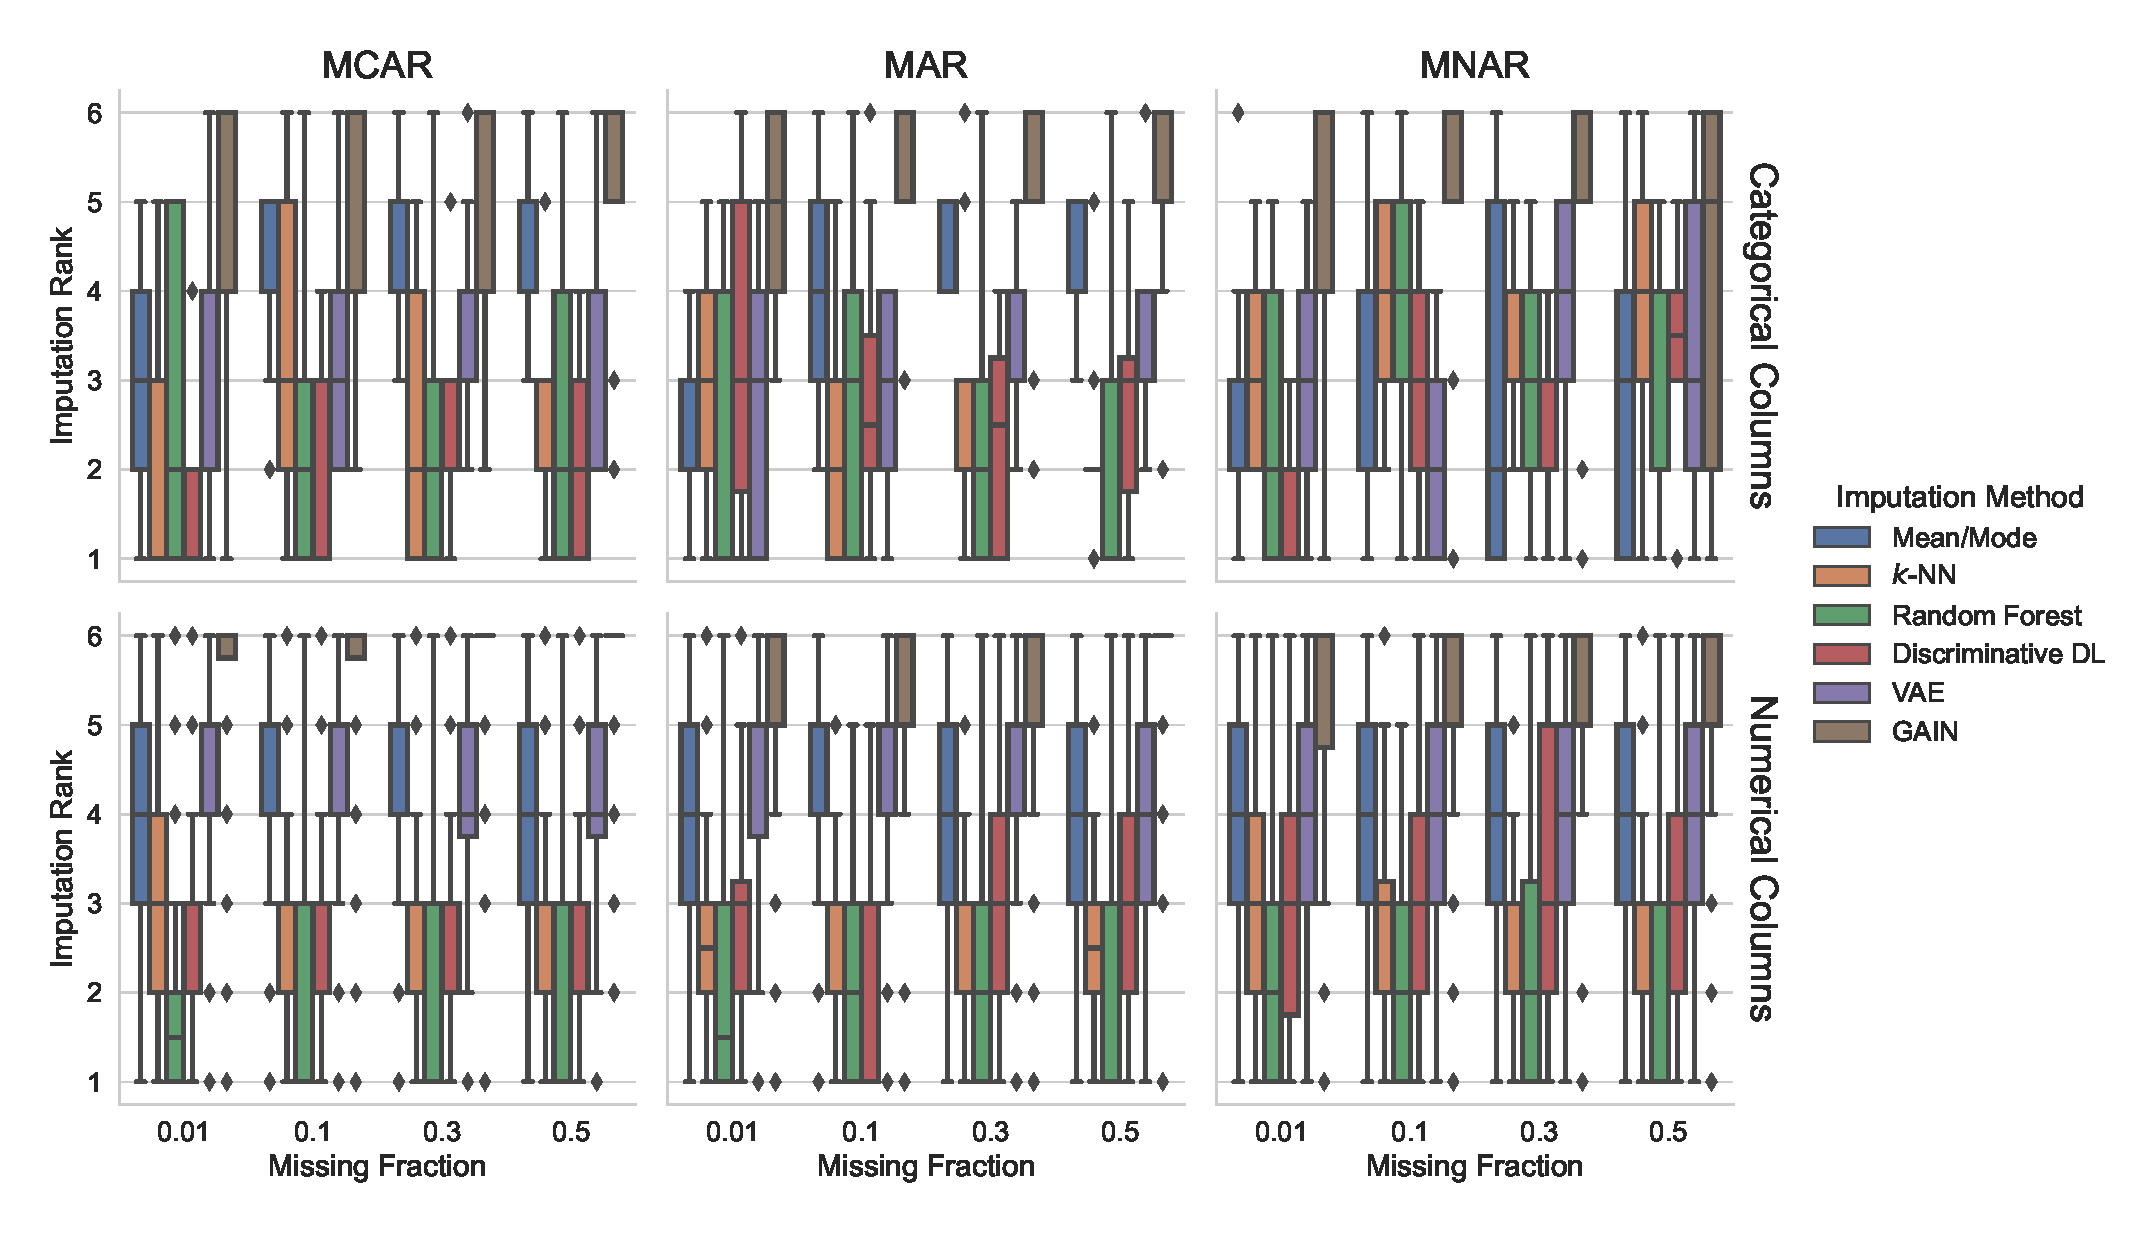
\includegraphics[width=1\columnwidth]{fully_observed_impute_rank_boxplot.eps}
    \caption[Imputation Ranks - Fully Observed]{Imputation quality of the six imputation methods trained on complete data. We plot the imputation method's rank against the missingness fraction. The columns of plots separate the changing missingness pattern, whereas the rows distinguish the results between categorical and numerical target columns. ML methods and discriminative DL tend to perform best. From left to right, we observe more variance (larger boxes), indicating that the results are less clear. Especially for categorical columns with the MNAR pattern and higher missingness fractions, mean/mode seems to be a good alternative.
	}
	\label{fig:fully_observed_impute_rank_boxplot}
\end{figure}

Figure \ref{fig:fully_observed_impute_rank_boxplot} shows the aggregated ranks for imputation performance when imputation methods are trained on fully observed data.

When imputing categorical columns, there is no clear winner. However, the discriminative DL approach yields high imputation quality in most cases. In the MAR setting, also the methods random forest and $k$-NN are often among the first two to three ranks. With increasing complexity the DL based methods seem to improve. Notably mean/mode imputation compares favorably in many cases especially in the most complex MNAR setting. In most cases GAIN appears to perform worse than other methods. As mentioned above, we can attribute this poor performance in part to a large proportion (33\%) of failed runs of in the current experiment/scenario, in which case GAIN was ranked last. However, in the setting of highest complexity (MNAR with 50\% missing values) the results of GAIN seem to improve.

When imputing numerical columns the differences are more pronounced. Random forest is the only method with 75\% of values, i.e. data sets, among the first three ranks throughout all experimental conditions. However, the whiskers indicate that there are also some results ranging on the middle and even last ranks. In most settings, $k$-NN ranks second or third on $50\%$ of the data sets, with tendencies to better ranks. Discriminative DL is almost as strong. Mean/mode and VAE's ranks are similarly distributed over all ranks with tendency to worse performances. For easier settings, such as MCAR and MAR with smaller missingness fractions, mean/mode tends to be better than VAE. Again, GAIN performs worst, this time even more clearly.

To summarize, classical ML methods and discriminative DL perform best when imputing missing values. However, for categorical columns in the MNAR setting there is often no improvement over mode imputation. The generative methods are mostly outperformed even by mean/mode with VAE not as clearly as GAIN.


\subsubsection{Scenario 2: Training on Incomplete Data}


\begin{figure}\centering
    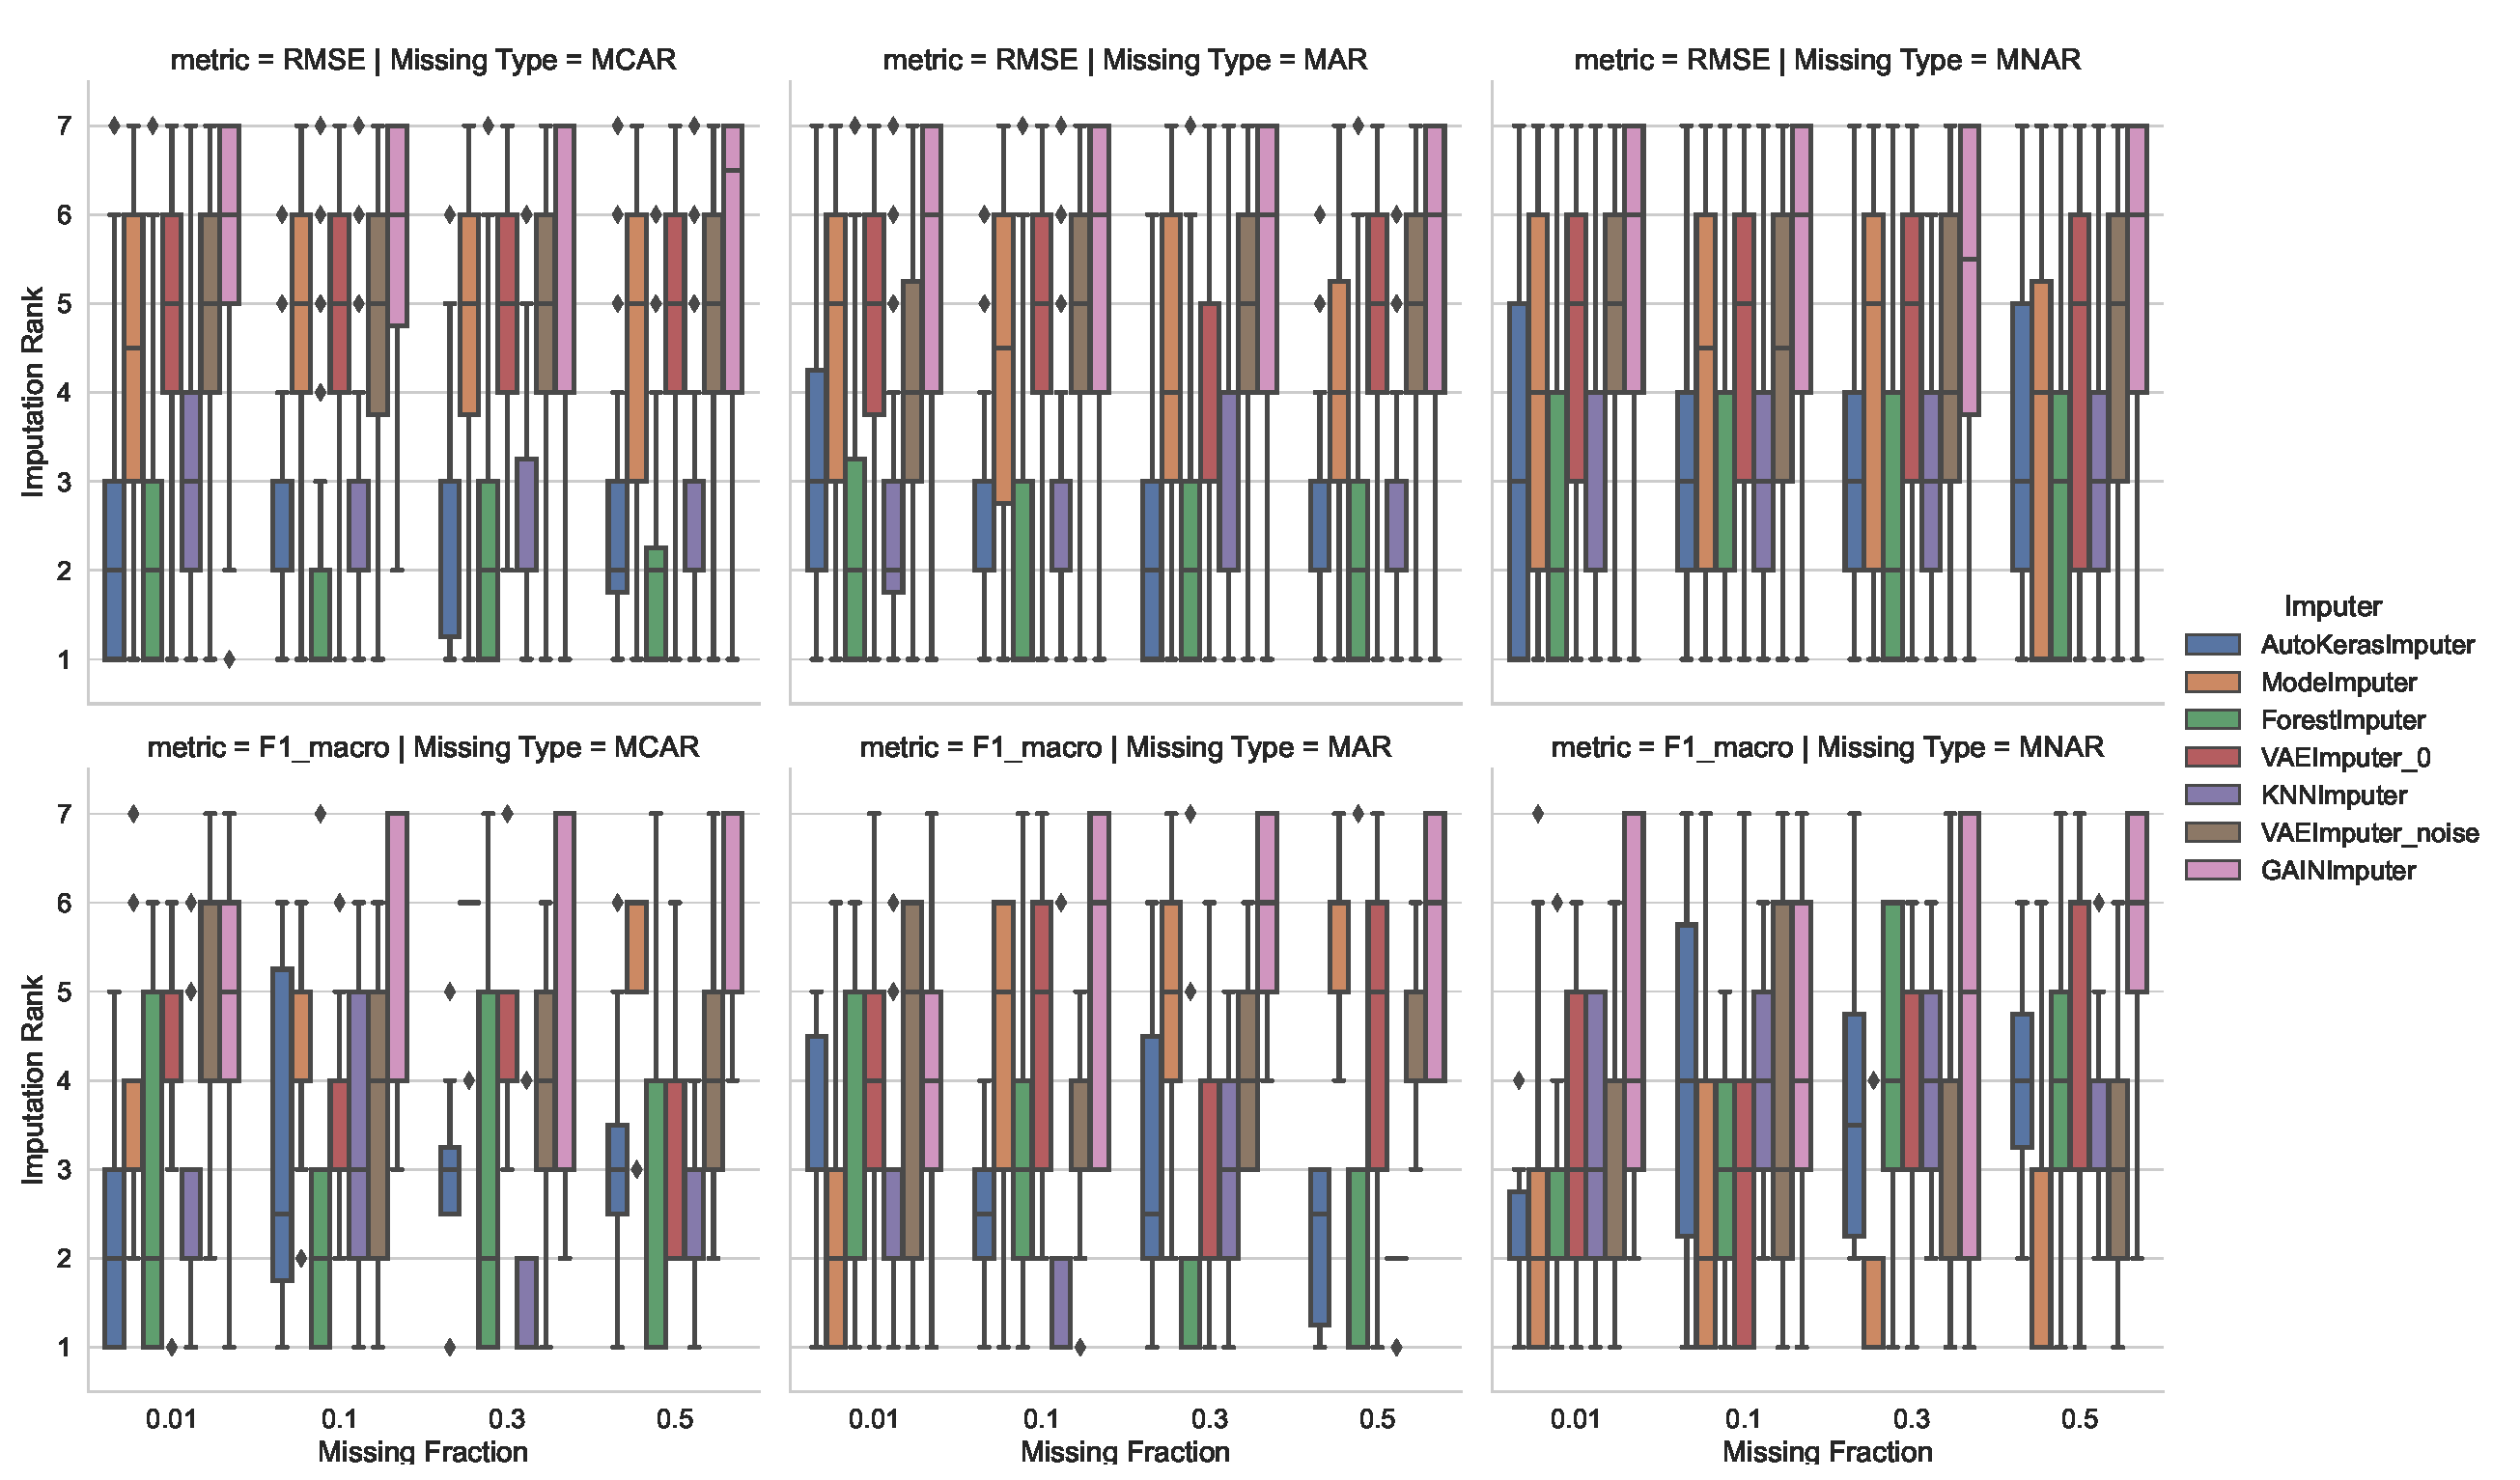
\includegraphics[width=1\columnwidth]{corrupted_impute_rank_boxplot.eps}

    \caption[Imputation Ranks - Corrupted]{Imputation quality of the six imputation methods trained on incomplete data. We plot the imputation method's rank against the missingness fraction. The columns of plots separate the changing missingness pattern, whereas the rows distinguish the results between categorical and numerical target columns. ML methods and discriminative DL tend to perform best. However, for categorical columns in the MNAR setting, there is often no improvement over mode imputation. \arndt{@Sebastian: ich finde, den letzten Satz kann man schon so schreiben im Bezug auf MNAR. Oder würdest du den weglassen?}
    }
	\label{fig:corrupted_impute_rank_boxplot}
\end{figure}

\autoref{fig:corrupted_impute_rank_boxplot} shows the imputation performance in \textit{Scenario 2}, i.e. when training on incomplete data. For categorical columns it is even harder to find clear patterns. With increasing task difficulty, the rank of the mean/mode imputation improves, though with higher variance. Interestingly, Mode imputation outperforms other methods especially in the most challenging settings (MNAR with 30\% and 50\% missing values). The methods $k$-NN and random forest compare favorably in the MCAR and MAR setting, but random forest has much higher variance. Discriminative DL yields similar performance in these settings, slightly worse on average and with lower variance than random forest. For MCAR and MAR these three methods tend to yield better performance than using Mean/Mode imputation, especially with an increasing fraction of missing values. The generative models tend to perform worst, especially GAIN.

Similar to the fully observed training case (Section \ref{sec:results_experiment1_scenario1}), imputation on numerical columns yields a clearer ranking than for categorical missing values. The imputation models $k$-NN and random forest yield best performances with a tendency of random forest to outperform $k$-NN, with larger variance of random forest. The Discriminative DL approach yields similar performance to the classical ML approaches in the MCAR and MAR settings. In the more challenging MNAR setting it performs slightly worse. Mean imputation and VAE perform comparably but worse than k-NN and Random Forest. GAIN falls on the last rank in most cases also in this setting.

Overall, the results of \textit{Scenario 1} (Figure \ref{fig:fully_observed_impute_rank_boxplot}) and \textit{Scenario 2} (Figure \ref{fig:corrupted_impute_rank_boxplot}) for numeric columns are quite similar. GAIN has become somewhat better in Scenario 2, although it still ranks worst. For categorical columns, the visualizations of the two scenarios are more pronounced in the incomplete training data setting. Whether imputation methods are trained on complete or incomplete data makes little difference in the ranks. The more difficult the task, depending on missingness pattern and fraction, the more ambiguous the results (higher variance). Classic ML methods like $k$-NN and random forest are generally a good choice. But also mean/mode yields relatively good results, especially when problems become more complex or the data is incomplete.


\subsection{Experiment 2: Impact on Downstream Task}

In this experiment we evaluate the downstream performance of each method when training on fully observed data and incomplete data.

In \textit{Scenario 1} we use the definition for \textit{impact on downstream task} from \autoref{eq:impact}. In contrast, for \textit{Scenario 2} we use the slightly different definition from \autoref{eq:impact_scenario2}. Both of theses metrics are labeled \textit{Improvement} and the values represented on the Y-axis in \autoref{fig:fully_observed_downstream_boxplot} and \autoref{fig:corrupted_downstream_boxplot}.

Experiemental settings that caused undefined results in the first experiment were filtered out in the second experiment. This means in particular that we have fewer results for GAIN in \textit{Scenario 1}.

\sebastian{Würde auch hier erst eine allgemienere einführugnen machen: Zeigen hier die Improvement berechnert wie in equation 3 o. 4 depending on scenario. Dass wir jetzt oben Classificaiton tasks und unten Regression haebn... UND: vor allem muss hier hien, dass wir jetzt nur noch die verwenden, die auch wirklich sinnvolle ergebnisse geliefert haben, also bein GAIN einiges fehlt.}

\felix{we should highlight the limitations of our results (only one column, maybe too simple)}


\subsubsection{Scenario 1: Training on Complete Data}

\sebastian{GANZ WICHTIG: wir haben hier keine infos darüber, welche columns imputed wurden. Was wir sehen ist ne Gruppierung nach Downstream task! - Ich würde da noch etwas weiter raus zoom am anfang: Allgemien, mehr missingness fürht zu mehr variance in der improvement. Überraschenderweise für calssification in beide Richtugnen aber deutliche tendenz für improvement und wieder wie oben RF/KNN/DL und Mean/mode sind ganz gut.. Regression fast ausschließlich improvements und wieder das bekannte trio am besten im regelfall.. (Hbane wir ne idee warum classificaiotn auch schelcht wird und regression nicht?)}


\begin{figure}\centering
	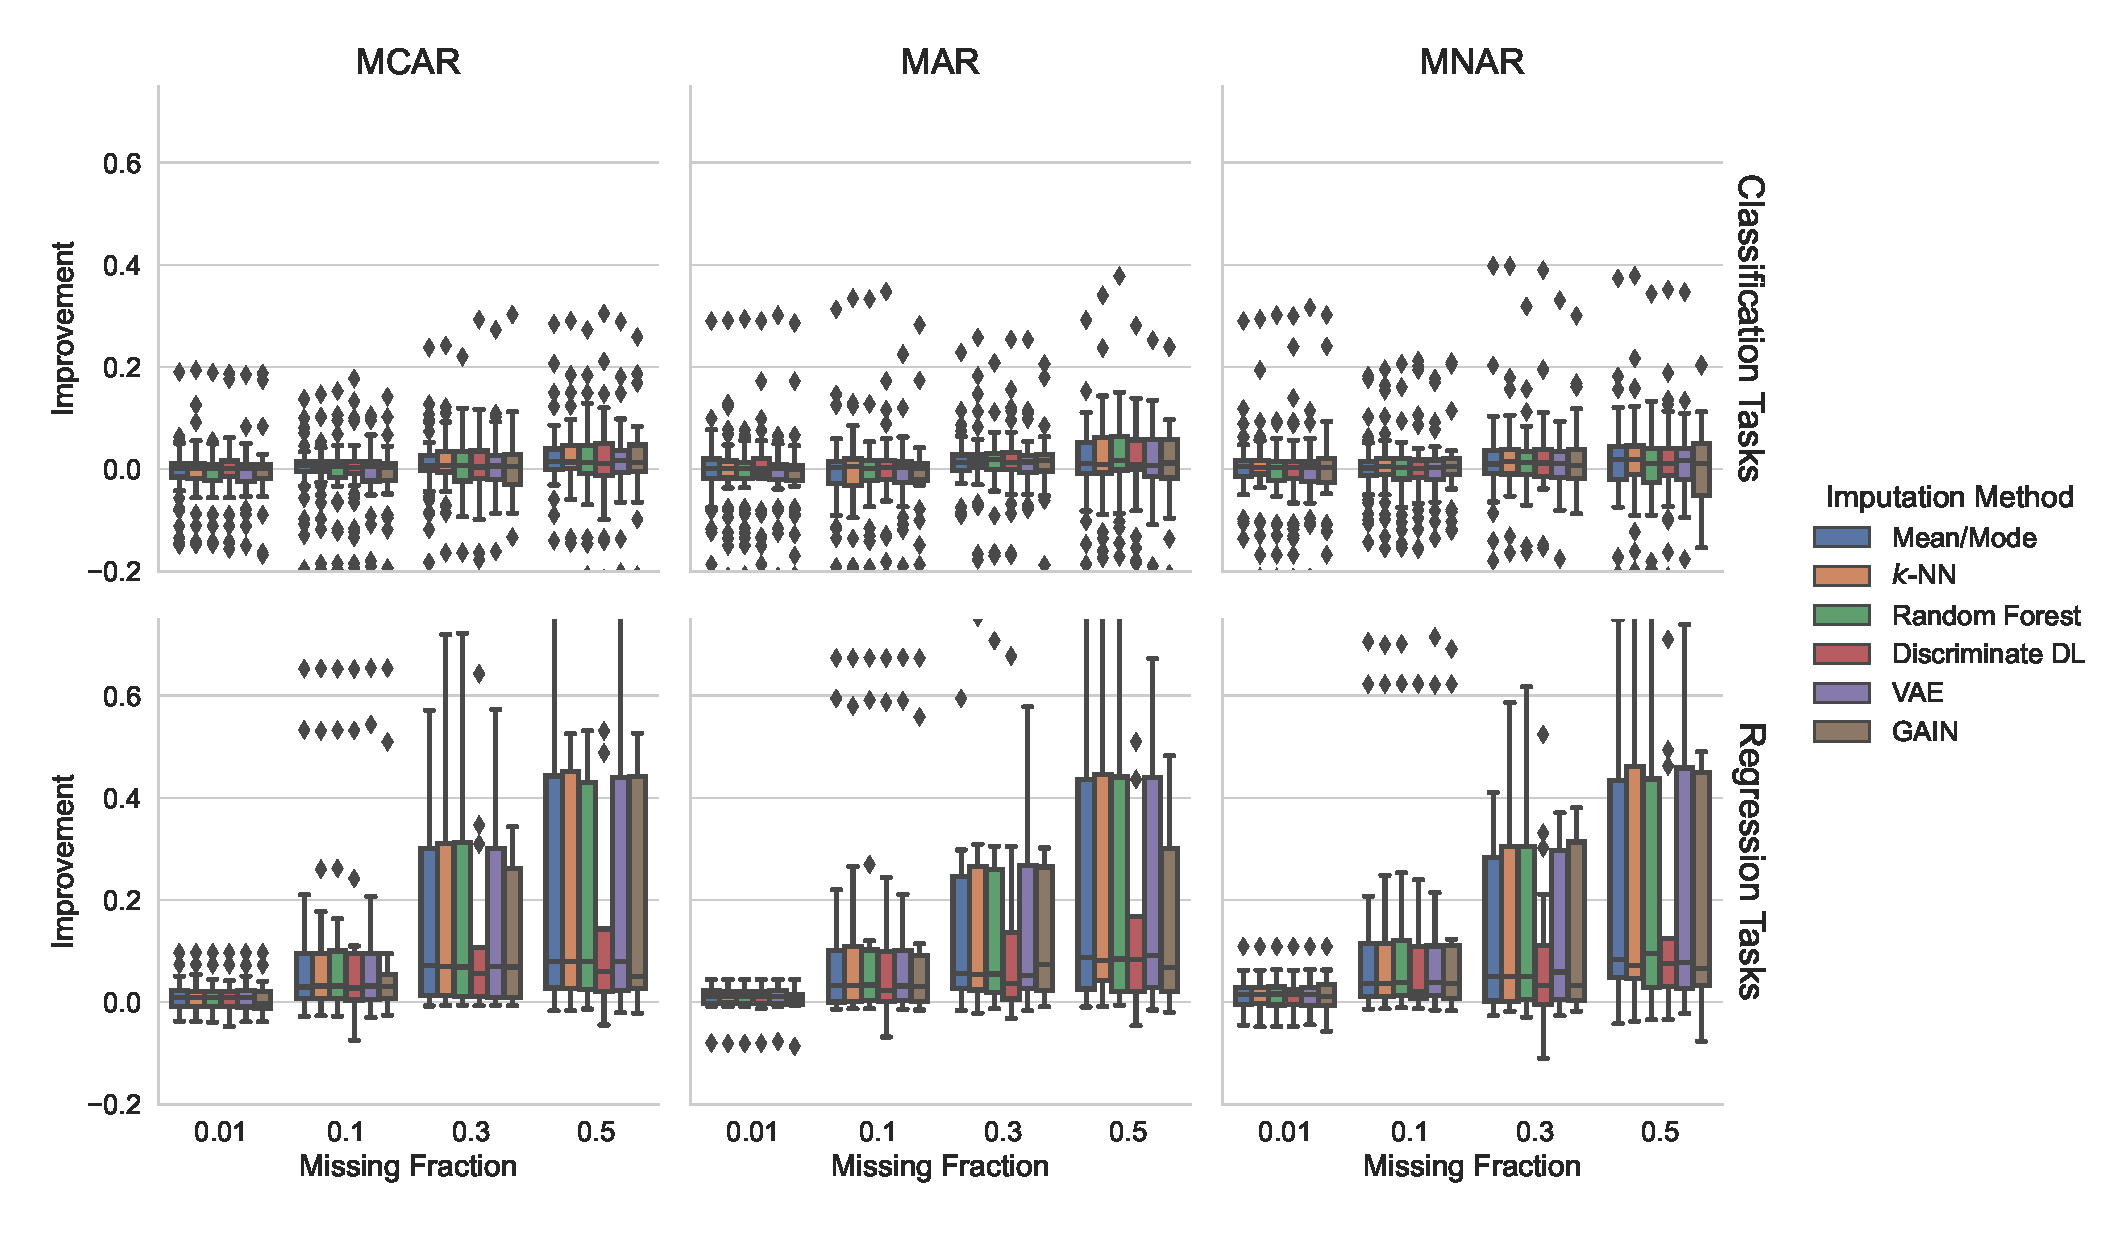
\includegraphics[width=1\columnwidth]{fully_observed_downstream_boxplot.eps}

	\caption[Downstream Ranks - Fully Observed]{Impact on downstream task of the six imputation methods trained on complete data. We plot the imputation method's rank against the missingness fraction. The columns of plots separate the changing missingness pattern, whereas the rows distinguish the results between categorical and numerical target columns. Overall, the classical ML methods and discriminative DL perform best.
    }
	\label{fig:fully_observed_downstream_boxplot}
\end{figure}

Figure \ref{fig:fully_observed_downstream_boxplot} visualizes the \textit{impact on downstream task} metric (Equation \ref{eq:impact}) in \textit{Scenario 1}. \arndt{hier ggf. in einem Satz nochmal zusammenfassen, wie die Berechnung erfolgt (sinngemäß).}

The impact of imputation seems mostly negligible if the proportion of missing values is only 1\%. However, for numeric columns, there are some outliers in the 20\% to 40\% improvement range with the MCAR and MAR patterns at 1\% missing values. With an increasing proportion of missing values we observe increasing improvements in the downstream performance in all types of missingness patterns. However, there are also some cases where downstream performance is degraded by imputation, which is mainly the case for categorical columns.

For categorical columns, improvements are mostly in the 0\% to 5\% range, and in case of 50\% missing values the upper quartile reaches the 5\% to 10\% range. The whiskers even indicate performance increases which go significantly beyond. Measured by the median, as an overall aggregation, Random Forest yields the best results for categorical columns. GAIN performs often similarly well or even better but also has more negative fluctuations.

The situation is different for regression tasks. Here, GAIN clearly yields the least improvements downstream. Even the Mean imputation is oftentimes significantly more beneficial for the downstream tasks. The VAE results are approximately on par with Mean imputation. In contrast, the classical ML and the discriminative DL approaches do outperform the other methods in most settings. However, when the missing values are MNAR there is no clear advantage except that the discriminative DL is superior at 50\% missing values.

Overall, the classical ML methods and discriminative DL perform best. As the proportion of missing values increases, we observe increasing improvements in all types of missingness patterns, along with higher variance, in downstream performance. In contrast to classification tasks, there are hardly any negative effects in regression tasks.

\subsubsection{Scenario 2: Training on Incomplete Data}

\sebastian{Auch hier: variance wird größer, wenn fraciton steigt. Jetzt aber tendenziell verschlechterungen.. Wieder aber für Regression besser als für classification. Mit KNN/Forest beste cahnce auf verbesserung.}


\begin{figure}\centering
	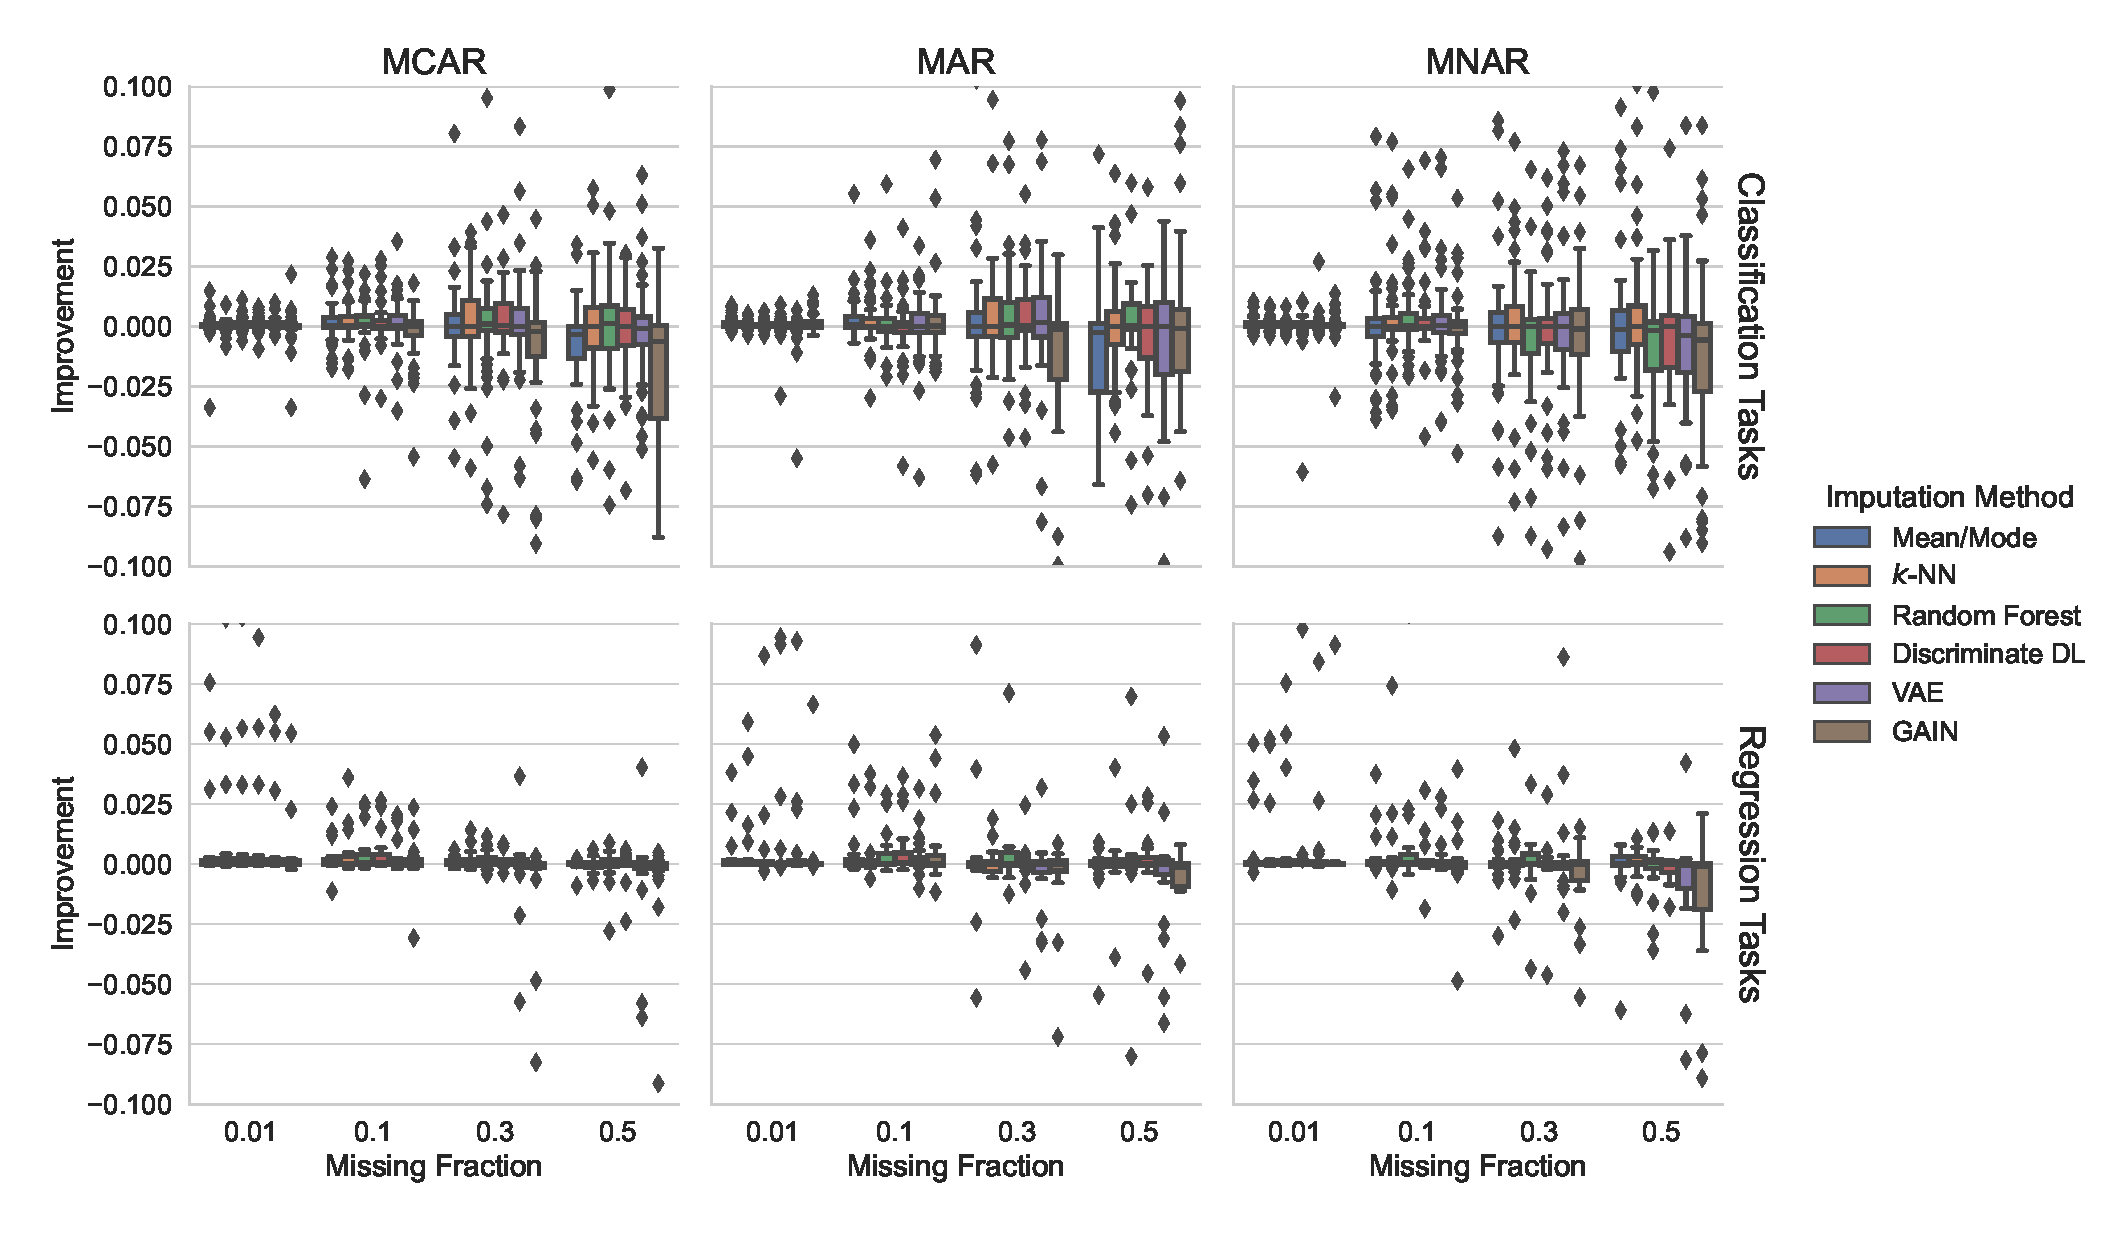
\includegraphics[width=1\columnwidth]{corrupted_downstream_boxplot.eps}

	\caption[Downstream Ranks - Corrupted]{Impact on downstream task of the six imputation methods trained on incomplete data. We plot the imputation method's rank against the missingness fraction. The columns of plots separate the changing missingness pattern, whereas the rows distinguish the results between categorical and numerical target columns. In regression tasks, no considerable improvements are achieved. In classification tasks, in contrast, we observe slightly positive effects in some settings but negative effects predominate in the harder settings.
    }
	\label{fig:corrupted_downstream_boxplot}
\end{figure}

Figure \ref{fig:corrupted_downstream_boxplot} illustrates the \textit{impact on downstream task} (Equation \ref{eq:impact_scenario2}) in \textit{Scenario 2} (training on incomplete/imputed data). Here, the different scaling of the y-axis must be taken into account, i.e. the relative improvements are significantly smaller compared to the first scenario. One reason for this is the different basis for calculating the relative values (see sections \ref{sec:experiment_2} and \ref{sec:scenario_2}).

If weak positive effects seem to predominate in classification tasks at first, this tendency changes with increasing proportion of missing values (at 50\%) and increasing difficulty of the task (especially MNAR). The most negative results are produced by GAIN. However, the other methods also have major difficulties and often drift into negative ranges for the greater part as the tasks become more challenging.

In regression tasks, apart from a few outliers, there are no significant improvements. At the highest proportion of missing values (50\%) and greatest difficulty (MNAR), the results of the generative methods (VAE and GAIN) even turn predominantly negative.

In summary, no considerable improvements were achieved in regression tasks. In classification tasks, the picture is more mixed and the variance is higher. In some settings, there are slightly positive effects to note. In the difficult settings, however, the negative effects predominate.

\arndt{consider points below in discussion}
\felix{
\begin{itemize}
\item in the conclusion we should relate the performance to the training and prediction time and comment on the (large) differences - for AutoKeras, a lot more tuning is performed and we don't know whether it would have worked as well with less tuning.
\item we should highlight the limitations of our results (only one column, maybe too simple)
\item we should highlight the main findings; as far as i can see this would be: a) classical methods perform best (on these simple (?) data sets) and b) downstream performance is improved by X \% in Y \% of the experiments (we can use the quantiles in the boxplots) whereas when the imputation methods are trained on incomplete data, we cannot expect improvements.
\end{itemize}
}
\sebastian{
\begin{itemize}
\item Scenario 2: Training on Incomplete Data - Spätestens jetzt sollten wir mal ein wort darüber verlieren woran das liegen könnte: When eine category einfach häufiger ist, dann ist das meist ne recht guter guess. Das könnte dazu führen, dass die andere schlechter werden, weil die versuchen das intelligenter zu machen, aber einfach nicht genügend trainings daten haben um noch was sinnvolles zu lernen
\end{itemize}
}

\subsection{Training Time}

\begin{table}
	\centering
	\label{tab:time}
	\begin{tabular}{lrr}
		\toprule
		Imputation Method &  Training Time &  Relative Standard Deviation \\
		\midrule
		Mean/Mode &       0.005009 &                     0.656056 \\
		$k$-NN &      40.961577 &                     0.243020 \\
		Random Forest &     225.513999 &                     0.118707 \\
		Discriminative DL &    6285.017741 &                     0.424011 \\
		VAE &      71.685278 &                     0.107189 \\
		GAIN &     874.657293 &                     0.299608 \\
		\bottomrule
	\end{tabular}
	\caption{Training time for each imputation method in seconds. Training time is the mean overall experimental settings, experiments, and scenarios. The data set's size skews the standard deviation heavily, which is why we first compute the relative standard deviation for each imputation method on each data set separately and then average over the data sets.\felix{for knn the training time should be almost 0, right? maybe it would be good to have the inference/prediction times as well, if we have that? kNN should perform much worse here, and the winner should be RF, i'm assuming}}
\end{table}

%!TEX root = ../data-imputation.tex
\section{Conclusions}
\label{sec:conclusion}
%
To the best of our knowledge, this is the first benchmark that compares classical and modern imputation approaches on a large number of datasets under realistic missingness conditions with respect to the imputation quality and the impact on the predictive performance of a downstream ML model. We also evaluated how the results change when the imputation and downstream model were trained on incomplete data.

Our results can be summarized in two main findings. First we demonstrate that imputation helps to increase the downstream predictive performance substantially regardless the missingness conditions. When training data is fully observed improvements for classification tasks were in more than 75\% of the cases between $10\%$ and $20\%$ and for regression tasks around $15\%$.

Second we find that in almost all experiments, random forest-based imputation achieves the best imputation quality and consequently also on the most data sets the best improvements on the downstream predictive performance. This finding is in line with previous imputation benchmark research in more constrained experimental conditions, see also Section \ref{sec:related_work}. Yet, some aspects of these results appear at odds with some recent work on deep learning methods. While we are aware of the limitations of our experiments, see also Section \ref{sec:limitations}, we still argue that in order to better assess the value of most deep learning methods it is helpful to stress test these methods under realistic conditions in large unified benchmarks with heterogeneous data sets \citep{Sculley2018, Bender2021}.






\bibliographystyle{frontiersinSCNS_ENG_HUMS} % for Science, Engineering and Humanities and Social Sciences articles, for Humanities and Social Sciences articles please include page numbers in the in-text citations
%\bibliographystyle{frontiersinHLTH&FPHY} % for Health, Physics and Mathematics articles
\bibliography{data-imputation}

%%% Make sure to upload the bib file along with the tex file and PDF


\end{document}
